\section{Estimators versus the CRB (R3)}\label{sec:estimators}

All MC results in this section use $L=50$\,nm, $\fwhm=\pnum{fwhm_nm}\src{fwhm_nm}$\,nm, seed
$42$ and $10^4$ repetitions unless stated otherwise; standard errors (SE) of $\sigma$ are
nonparametric bootstrap estimates.

\emph{MLE with background: efficient at the centre.} With $\sbr=10$ the model is regular at the
centre ($p_3>0$). For $N=100$ and an MLE search disk of radius $L$, the MLE precision is
$\sigma=\pnum{mle_sigma_center_sbr10_nm}\pm\pnumse{mle_sigma_center_sbr10_nm}$\src{mle_sigma_center_sbr10_nm}\,nm
against the bound \pnum{crb_center_sbr10_L50_N100_nm}\src{crb_center_sbr10_L50_N100_nm}\,nm of
Eq.~\eqref{eq:s31}: an efficiency
$\sigma/\crb=\pnum{mle_efficiency_center}\pm\pnumse{mle_efficiency_center}$\src{mle_efficiency_center}.
This is the value we define as the MLE efficiency at the centre; the choice $\sbr=10$ (a
regular, physical case) is a declared convention (Sec.~\ref{sec:open}).

\emph{MLE without background: biased and superefficient.} Without background $p_3\propto r^2$,
the model is not regular at the centre, and the MLE beats the CRB limit:
$\sigma=\pnum{mle_nobg_sigma_center_nm}\pm\pnumse{mle_nobg_sigma_center_nm}$\src{mle_nobg_sigma_center_nm}\,nm,
i.e.\ $\sigma/\sigma_{\lim}=\pnum{mle_nobg_sigma_over_crb_limit_center}\pm\pnumse{mle_nobg_sigma_over_crb_limit_center}$\src{mle_nobg_sigma_over_crb_limit_center}
and $\sigma/\sigma_{\mathrm{pt}}=\pnum{mle_nobg_sigma_over_s27_center}\pm\pnumse{mle_nobg_sigma_over_s27_center}$\src{mle_nobg_sigma_over_s27_center}
at $N=100$. The ratio does not approach one as $N$ grows [Fig.~\ref{fig:estimators}(c)], so this
is not a small-$N$ effect. The price is a bias, toward the centre close to it
[for $x_0\lesssim8$\,nm, Fig.~\ref{fig:estimators}(d)]: at $\rr=(2,0)$\,nm the mean
error along $x$ is
$\pnum{mle_nobg_bias_x_r2_nm}\pm\pnumse{mle_nobg_bias_x_r2_nm}$\src{mle_nobg_bias_x_r2_nm}\,nm
($4\times10^4$ repetitions) [Fig.~\ref{fig:estimators}(d)]. The CRB bounds only unbiased
estimators of a regular model, so there is no contradiction; it means that, without background,
neither the point value nor the limit is a bound on what an MLE reports near the centre.

\emph{LMS.} Without background the LMS estimate at the centre has exactly the covariance of the
point value, $L^2/(8Ng^2)$ per axis\src{lms_center_analytic}: in MC,
$\sigma/\sigma_{\mathrm{pt}}=\pnum{lms_nobg_sigma_over_s27_center}\pm\pnumse{lms_nobg_sigma_over_s27_center}$\src{lms_nobg_sigma_over_s27_center}
and $\sigma/\sigma_{\lim}=\pnum{lms_nobg_sigma_over_crb_limit_center}\pm\pnumse{lms_nobg_sigma_over_crb_limit_center}$\src{lms_nobg_sigma_over_crb_limit_center}
($=1/\rho$), constant in $N$ [Fig.~\ref{fig:estimators}(c)]. With background, the expectation of the LMS of
Balzarotti Eq.~S50 without the $1/s$ correction is exactly $s=\sbr/(\sbr+1)$ times that of the
background-free LMS at every position\src{lms_sbr_shrink} (the constant background term cancels
because $\sum_k\bb_k=\mathbf0$). In Fig.~\ref{fig:estimators}(a,b) the LMS and mLMS include the
$1/s$ correction. Beyond $x_0\approx15$\,nm they are strongly biased toward the centre
[Fig.~\ref{fig:estimators}(a)], because the linearization compresses the estimate, and their
$\sigma$ falls below the CRB [Fig.~\ref{fig:estimators}(b)]; this reflects the compression, not a
gain in precision. Closer to the centre this does not hold: for $x_0\lesssim12$\,nm the mLMS has
$\sigma$ above the CRB, and for $x_0\approx5$--$15$\,nm its bias is small and slightly outward.

\emph{MLE away from the centre: an outlier tail at low $N$.} With $\sbr=10$ and $N=100$ the MLE
is not efficient everywhere inside the TCP. At $\rr=(15,0)$\,nm, with a search disk of radius
$2L$, $\sigma/\crb=\pnum{mle_sbr10_sigma_over_crb_x15_N100}\pm\pnumse{mle_sbr10_sigma_over_crb_x15_N100}$\src{mle_sbr10_sigma_over_crb_x15_N100},
caused by a tail of outliers (the bump in Fig.~\ref{fig:estimators}(b) for $x_0\approx10$--$20$\,nm);
at $N=1000$ it is
$\pnum{mle_sbr10_sigma_over_crb_x15_N1000}\pm\pnumse{mle_sbr10_sigma_over_crb_x15_N1000}$\src{mle_sbr10_sigma_over_crb_x15_N1000}.
The size of the tail depends on the search radius, which must therefore be reported with any
such number; the convergence of the MLE to the CRB away from the centre only at larger $N$ agrees
with Ref.~\cite{Balzarotti2017}.

\begin{figure*}[t]
\centering
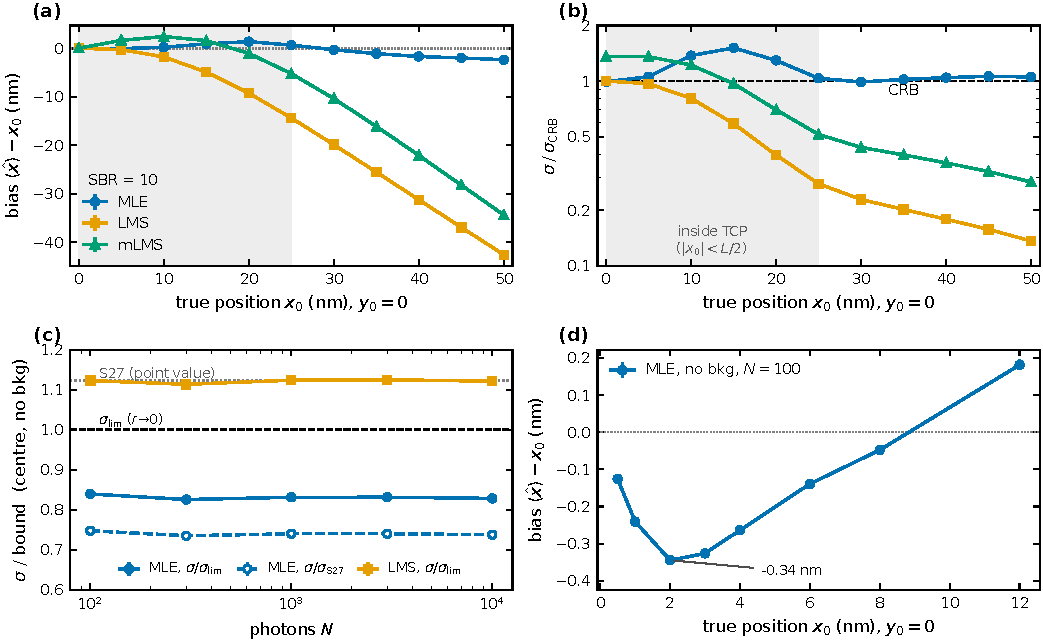
\includegraphics[width=\textwidth]{figures/fig5_estimators.pdf}
\caption{Estimators versus the CRB ($L=50$\,nm, $N=100$ unless indicated, seed 42).
(a)~Bias and (b)~$\sigma/\crb$ versus the emitter position $x_0$ along $x$, from the centre to
$L$ (inside the TCP shaded), for the MLE, the LMS and the mLMS with $\sbr=10$; off-centre MLE
points use a search disk of radius $2L$, and the centre point (radius $L$, $10^4$ repetitions)
equals the efficiency
$\pnum{mle_efficiency_center}\src{mle_efficiency_center}$. The MLE bump in (b) at
$x_0\approx10$--$20$\,nm ($\sigma/\crb=\pnum{mle_sbr10_sigma_over_crb_x15_N100}\src{mle_sbr10_sigma_over_crb_x15_N100}$
at $x_0=15$\,nm) is an outlier tail whose size depends on the $2L$ search radius. (c)~Centre,
no background: $\sigma$ of the MLE divided by the $r\to0$ limit (superefficiency,
\pnum{mle_nobg_sigma_over_crb_limit_center}\src{mle_nobg_sigma_over_crb_limit_center} at
$N=100$) and by the point value of Eq.~\eqref{eq:s27}
(\pnum{mle_nobg_sigma_over_s27_center}\src{mle_nobg_sigma_over_s27_center}), and $\sigma$ of the
LMS divided by the limit, versus $N$. (d)~Bias of the background-free MLE near the centre
versus $x_0$ ($N=100$): negative (toward the centre) for $x_0\lesssim8$\,nm, with
$\pnum{mle_nobg_bias_x_r2_nm}\pm\pnumse{mle_nobg_bias_x_r2_nm}$\src{mle_nobg_bias_x_r2_nm}\,nm
at $\rr=(2,0)$\,nm, and changing sign (away from the centre) near $x_0\approx9$\,nm.}
\label{fig:estimators}
\end{figure*}
